\item \textbf{{[}JPJC/PRELIM/9597/2019/P1/Q3{]} }

JP Medical Centre uses a priority queue to register patients who visit
for medical attention. Upon registration at the medical centre, each
patient will be assigned a priority number according to the urgency
in seeking medical care. The urgent cases receive top priority and
go directly to the front of the queue, whereas the minor cases are
added to the bottom of the queue.

A priority queue is an extension of queue with the following properties.
\begin{itemize}
\item Every element has a priority associated with it. Higher priority has
a larger number. 
\item An element with high priority leaves the queue before an element with
low priority.
\item If two elements have the same priority, they are served according
to their order in the queue, i.e. the earlier element will be served
before the later element (FIFO). 
\end{itemize}
An example of operations on a priority queue is shown below:

\textbf{Initial state of priority queue} 

\begin{tabular}{|c|c|c|c|c|c|}
\hline 
Data & \textquoteleft jim\textquoteright{} & \textquoteleft ben\textquoteright{} & \textquoteleft ken\textquoteright{} & \textquoteleft wayne\textquoteright{} & \textquoteleft harry\textquoteright{}\tabularnewline
\hline 
Priority & 3 & 3 & 2 & 1 & 1\tabularnewline
\hline 
\multicolumn{1}{c}{} & \multicolumn{1}{c}{$\overset{\uparrow}{\boldsymbol{\text{front}}}$} & \multicolumn{1}{c}{} & \multicolumn{1}{c}{} & \multicolumn{1}{c}{} & \multicolumn{1}{c}{$\overset{\uparrow}{\boldsymbol{\text{rear}}}$}\tabularnewline
\end{tabular}

\textbf{Insert \textquoteleft jenny\textquoteright{} with priority
3:} \textquoteleft jenny\textquoteright{} joins the priority queue
ahead of \textquoteleft ken\textquoteright{} who has a priority of
2 

\begin{tabular}{|c|c|c|c|c|c|c|}
\hline 
Data & \textquoteleft jim\textquoteright{} & \textquoteleft ben\textquoteright{} & '\emph{jenny}' & \textquoteleft ken\textquoteright{} & \textquoteleft wayne\textquoteright{} & \textquoteleft harry\textquoteright{}\tabularnewline
\hline 
Priority & 3 & 3 & \emph{3} & 2 & 1 & 1\tabularnewline
\hline 
\multicolumn{1}{c}{} & \multicolumn{1}{c}{$\overset{\uparrow}{\boldsymbol{\text{front}}}$} & \multicolumn{1}{c}{} & \multicolumn{1}{c}{} & \multicolumn{1}{c}{} & \multicolumn{1}{c}{} & \multicolumn{1}{c}{$\overset{\uparrow}{\boldsymbol{\text{rear}}}$}\tabularnewline
\end{tabular}

Remove from priority queue: \textquoteleft jim\textquoteright{} is
removed from front of priority queue 

\begin{tabular}{|c|c|c|c|c|c|}
\hline 
Data & \textquoteleft ben\textquoteright{} & '\emph{jenny}' & \textquoteleft ken\textquoteright{} & \textquoteleft wayne\textquoteright{} & \textquoteleft harry\textquoteright{}\tabularnewline
\hline 
Priority & 3 & \emph{3} & 2 & 1 & 1\tabularnewline
\hline 
\multicolumn{1}{c}{} & \multicolumn{1}{c}{$\overset{\uparrow}{\boldsymbol{\text{front}}}$} & \multicolumn{1}{c}{} & \multicolumn{1}{c}{} & \multicolumn{1}{c}{} & \multicolumn{1}{c}{$\overset{\uparrow}{\boldsymbol{\text{rear}}}$}\tabularnewline
\end{tabular}

A \textbf{priority queue} abstract data type (ADT) is to be \textbf{implemented}
as \textbf{a linked list} using object-oriented programming. Two classes
\texttt{Node} and \texttt{PQueue} have been identified. 
\begin{center}
\begin{tabular}{|l|l|l|}
\hline 
\multicolumn{3}{|c|}{\texttt{Class: Node}}\tabularnewline
\hline 
\texttt{\textbf{\hspace{0.01\columnwidth}}}\textbf{Identifier} & \texttt{\textbf{\hspace{0.01\columnwidth}}}\textbf{Data Type} & \texttt{\textbf{\hspace{0.05\columnwidth}}}\textbf{Description}\tabularnewline
\hline 
\multicolumn{3}{|l|}{\textbf{Properties}}\tabularnewline
\hline 
\texttt{Data} & \texttt{STRING} & The node data\tabularnewline
\hline 
\texttt{Priority} & \texttt{INTEGER} & Indicates priority of node. Higher value has higher priority.\tabularnewline
\hline 
\texttt{Pointer} & \texttt{INTEGER} & Pointer to next node in queue.\tabularnewline
\hline 
\end{tabular}
\par\end{center}

\begin{center}
\begin{tabular}{|l|l|l|}
\hline 
\multicolumn{3}{|c|}{\texttt{Class: PQueue}}\tabularnewline
\hline 
\texttt{\textbf{\hspace{0.01\columnwidth}}}\textbf{Identifier} & \texttt{\textbf{\hspace{0.01\columnwidth}}}\textbf{Data Type} & \texttt{\textbf{\hspace{0.05\columnwidth}}}\textbf{Description}\tabularnewline
\hline 
\multicolumn{3}{|l|}{\textbf{Properties}}\tabularnewline
\hline 
\texttt{ThisPQueue} & \texttt{ARRAY{[}10{]} OF Node} & The data for the priority queue.\tabularnewline
\hline 
\texttt{Front} & \texttt{INTEGER} & Index for front node of queue. \tabularnewline
\hline 
\texttt{Rear} & \texttt{INTEGER} & Index for rear node of queue. \tabularnewline
\hline 
\texttt{NextFree} & \texttt{INTEGER} & Index for the next unused node.\tabularnewline
\hline 
\multicolumn{3}{|l|}{\textbf{Methods}}\tabularnewline
\hline 
\multirow{2}{*}{Initialise} & \multirow{2}{*}{\texttt{PROCEDURE}} & \textbullet{} Create a new priority queue \tabularnewline
 &  & \textbullet{} Initialise \texttt{Front} and \texttt{Rear} to -1.\tabularnewline
\hline 
\multirow{3}{*}{\texttt{JoinPQueue (NewItem:STRING, Priority:INTEGER)}} & \multirow{3}{*}{\texttt{PROCEDURE}} & \textbullet{} Create a new node of Node class.\tabularnewline
 &  & \textbullet{} Assign \texttt{NewItem} and \texttt{Priority} passed
as parameters to the \texttt{Data} and \texttt{Priority} attribute
of \texttt{Node}.\tabularnewline
 &  & \textbullet{} Assign \texttt{Node} to the \texttt{PQueue} according
to the priority of the node.\tabularnewline
\hline 
\multirow{2}{*}{\texttt{LeavePQueue}} & \multirow{2}{*}{\texttt{FUNCTION}} & \textbullet{} Remove \texttt{Node} from \texttt{PQueue}.\tabularnewline
 &  & \textbullet{} Return the \texttt{data} attribute of \texttt{Node}. \tabularnewline
\hline 
\end{tabular}
\par\end{center}

The diagram shows the linked list with: 
\begin{itemize}
\item the elements \textquoteleft ben\textquoteright , \textquoteleft jenny\textquoteright ,
\textquoteleft ken\textquoteright , \textquoteleft wayne\textquoteright ,
\textquoteleft harry\textquoteright{} in the priority queue
\item the unused nodes linked together
\end{itemize}
\begin{center}
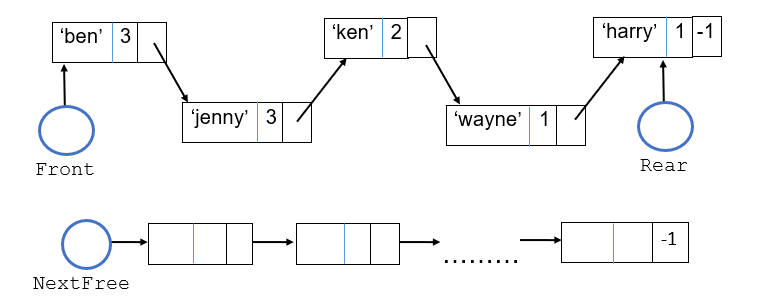
\includegraphics[width=0.65\paperwidth]{C:/Users/Admin/Desktop/Github/question_bank/LyX/static/img/9597-JPJC-2019-P1-Q3-1}
\par\end{center}

\subsection*{Task 3.1 }

Write program code to
\begin{itemize}
\item declare all the required identifiers for the \texttt{Node} and \texttt{PQueue}
class as specified, including the methods \texttt{Initialise}, \texttt{JoinPQueue},
\texttt{LeavePQueue}, and 
\item create the initial priority queue. 
\end{itemize}

\subsection*{Evidence 6: }

Your program code. \hfill{}{[}25{]}

\subsection*{Task 3.2 }

Write a procedure \texttt{OutputQueue} which displays the value of
\texttt{Front}, \texttt{Rear}, and \texttt{NextFree} and the contents
of \texttt{ThisPQueue} in index order. 

\subsection*{Evidence 7: }
\begin{itemize}
\item Your program code for \texttt{OutputPQueue}.
\item Screenshot for displaying the initial priority queue. \hfill{}{[}4{]}
\end{itemize}

\subsection*{Task 3.3 }

Write a main program to:
\begin{itemize}
\item Read from file\texttt{ PATIENTS.txt} all the data items with its priorities
into the priority queue by calling procedure \texttt{JoinPQueue}.
\item Output the priority queue by calling \texttt{OutputPQueue}. 
\end{itemize}

\subsection*{Evidence 8: }
\begin{itemize}
\item Your program code for task 3.3. 
\item Screenshot showing the output from running program in task 3.3. \hfill{}{[}5{]}
\end{itemize}
Task 3.4 

Write additional code in your main program that prints a menu with
the following options:

\noindent\fbox{\begin{minipage}[t]{1\columnwidth - 2\fboxsep - 2\fboxrule}%
\noindent \texttt{Patient Queue Menu }
\begin{enumerate}
\item[1)] \texttt{ Add patient to PQueue }
\item[2)] \texttt{ Remove patient from PQueue }
\item[3)] \texttt{ Display PQueue }
\item[4)] \texttt{ Exit program }
\end{enumerate}
%
\end{minipage}}

Write program code for each option by calling the appropriate methods
from the \texttt{PQueue} class. 

\subsection*{Evidence 9: }

Your program code for task 3.4.\hfill{} {[}4{]}

\subsection*{Task 3.5 }

Test your main program by doing the following in order and display
the priority queue: 
\noindent \begin{center}
\begin{tabular}{|l|l|l|l|}
\hline 
No. & Operation & Data  & Priority\tabularnewline
\hline 
1 & Remove patient & - & -\tabularnewline
\hline 
2 & Add patient & Donny & 2\tabularnewline
\hline 
\end{tabular} 
\par\end{center}

\subsection*{Evidence 10: }

Screenshot for testing your program in task 3.5.\hfill{} {[}2{]}